% Results
\section{Hasil dan Pembahasan}
Bagian ini menyajikan hasil analisis data serta interpretasi dari temuan penelitian. Hasil yang diperoleh dari proses klasterisasi, evaluasi, dan visualisasi akan dibahas secara sistematis.

\subsection{Hasil Klasterisasi}
Berdasarkan \textit{Elbow Method} (Grafik~\Ref{fig:elbowmethod}) dan \textit{Gap Statistics} (Grafik~\Ref{fig:gapstat}), jumlah cluster optimal ditentukan sebanyak tiga. Walaupun terdapat elbow di angka 6 dan 9, angka 3 dipilih karena angka lebih dari 3 akan menyebabkan overfitting. Overfitting biasanya menyebabkan penurunan akurasi pada model (\cite{Webb2011}). Setelah proses \textit{scaling} dan penerapan \textit{K-Means}, didapatkan hasil distribusi mahasiswa ke dalam 3 cluster sebagai berikut:
\begin{table}[!htpb]
    \centering
    \caption{Distribusi Mahasiswa pada Setiap Cluster}
    \label{tab:cluster-distribusi}
    \begin{tabular}{lccccccc}
        \hline
        \textbf{Cluster} & \textbf{Last} & \textbf{Overall} & \textbf{Attendance\_num} & \textbf{Gaming\_num} & \textbf{Preparation\_num} & \textbf{Computer} & \textbf{Income\_num} \\
        \hline
        1 & 3.52 & 3.52 & 3.56 & 2.29 & 1.92 & 3.57 & 2.59 \\
        2 & 2.50 & 2.57 & 2.56 & 2.95 & 1.18 & 3.11 & 2.71 \\
        3 & 3.54 & 3.53 & 3.66 & 2.16 & 1.86 & 2.92 & 2.24 \\
        \hline
    \end{tabular}
\end{table}

Pemilihan kolom yang pada Tabel~\ref{tab:cluster-distribusi} berdasarkan hasil visualisasi kontribusi tiap fitur.
\pagebreak

\begin{figure}[!htpb]
    \centering
    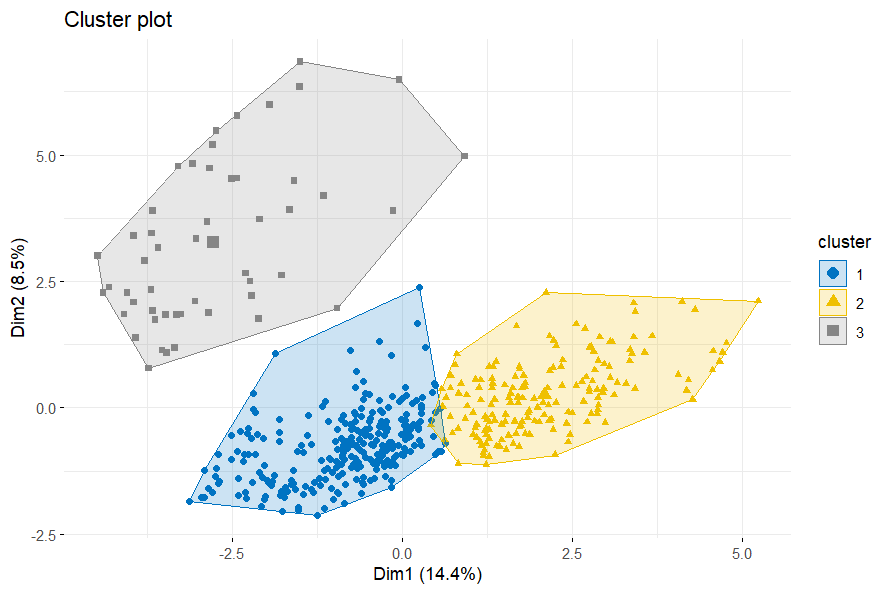
\includegraphics[width=0.8\textwidth]{figures/clusterplot.png}
    \caption{Visualisasi hasil klasterisasi mahasiswa}
    \label{fig:cluster-visualization-png}
\end{figure}

\begin{figure}[!htpb]
    \centering
    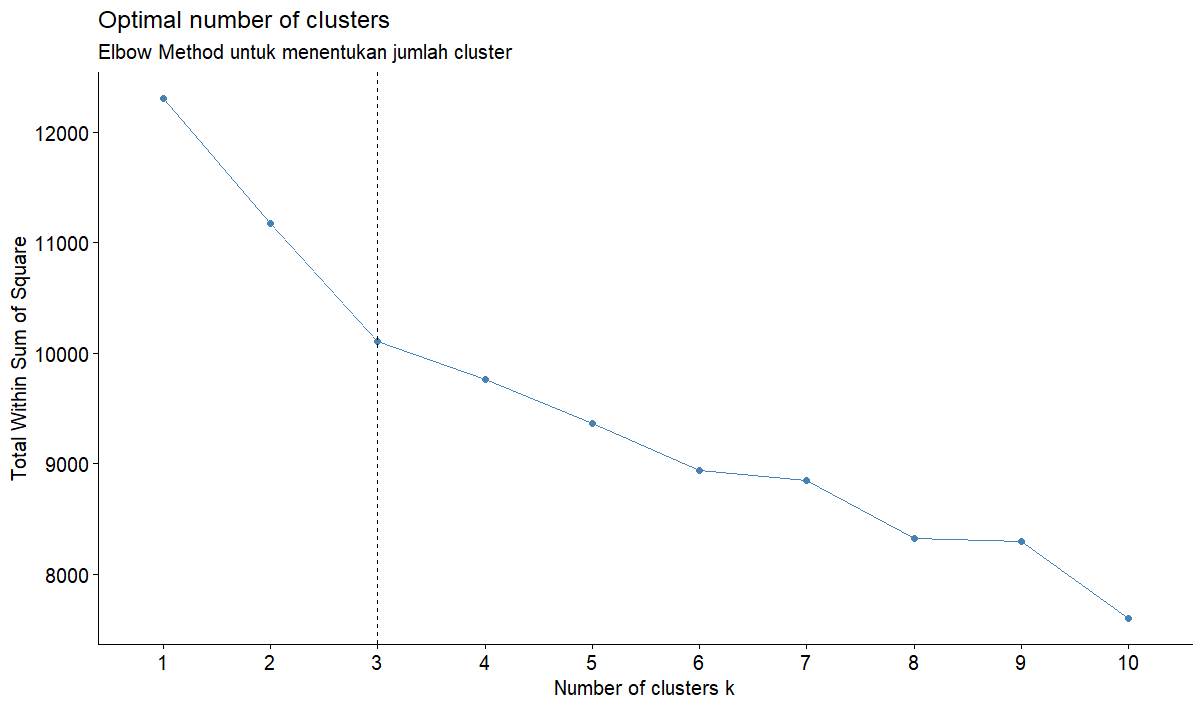
\includegraphics[width=0.8\textwidth]{figures/elbowmethod.png}
    \caption{Elbow Method}
    \label{fig:elbowmethod}
\end{figure}

\begin{figure}[!htpb]
    \centering
    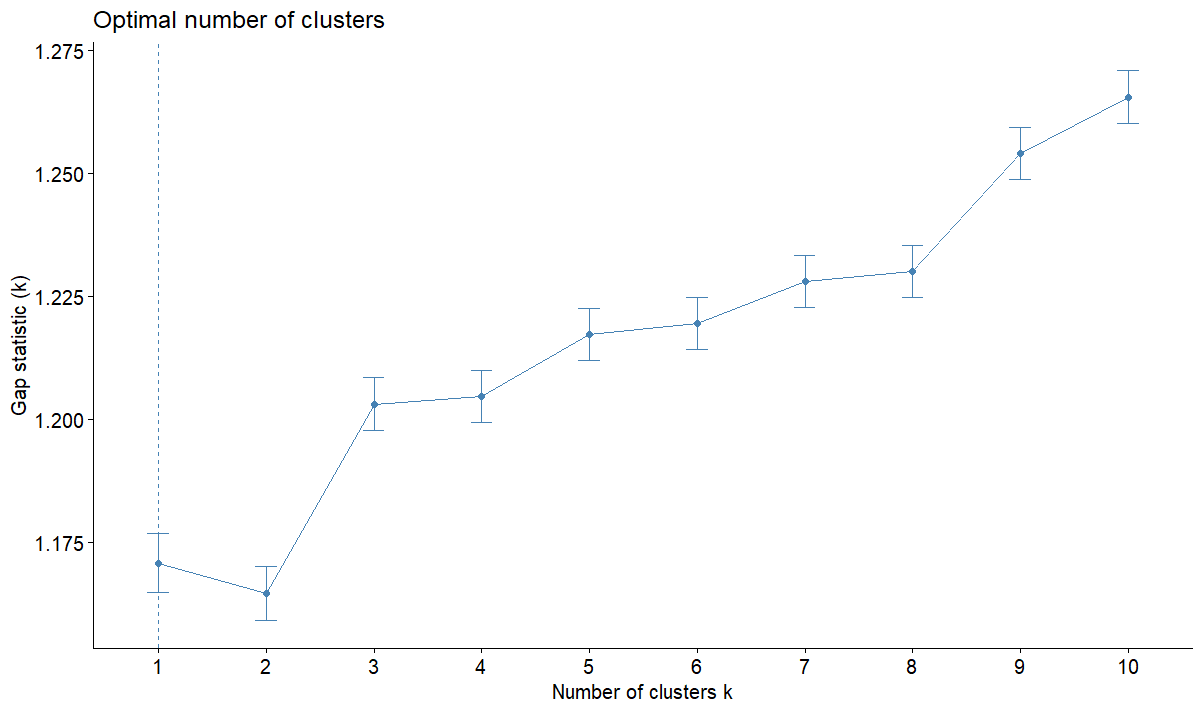
\includegraphics[width=0.8\textwidth]{figures/gapstat.png}
    \caption{Gap Statistics}
    \label{fig:gapstat}
\end{figure}
\pagebreak

\subsection{PCA}
Dataset terdiri dari 16 fitur, sehingga visualisasi biplot menjadi kurang jelas dan informatif jika semua fitur ditampilkan sekaligus (lihat Grafik~\ref{fig:biplotcluttered}). Oleh karena itu, biplot divisualisasikan dengan memisahkan fitur-fitur berdasarkan tema yang serupa. Berikut adalah hasil visualisasinya:
\begin{itemize}
    \item Grafik~\ref{fig:biplot-academic} menampilkan biplot yang hanya memuat fitur-fitur akademik, yaitu "HSC", "SSC", "Computer", "English", "Last", dan "Overall".
    \item Grafik~\ref{fig:biplot-habits} menampilkan biplot yang hanya memuat fitur-fitur kebiasaan dan demografi, yaitu "Preparation\_num", "Gaming\_num", "Attendance\_num", "Semester\_num", "Income\_num", "Job\_num", "Extra\_num", "Hometown\_num", dan "Gender\_num".
    \item Grafik~\ref{fig:biplot-department} menampilkan biplot berdasarkan variabel departemen masing-masing mahasiswa dalam dataset.
\end{itemize}

Berdasarkan Grafik~\ref{fig:cluster-contribution1} dan Grafik~\ref{fig:cluster-contribution2}, dapat dilihat bahwa fitur "Last", "Overall", "Attendance\_num", dan "Gaming\_num" memberikan kontribusi terbesar pada Dimensi 1, yang merepresentasikan aspek performa akademik mahasiswa. Sementara itu, Dimensi 2 memisahkan mahasiswa berdasarkan latar belakang departemen, khususnya antara kelompok STEM dan non-STEM. Hal ini juga tercermin pada Grafik~\ref{fig:biplotcluttered}, di mana panah fitur "Overall" dan "Last" mengarah ke kiri, sedangkan "Gaming\_num" mengarah ke kanan, mengindikasikan adanya hubungan negatif antara waktu bermain game dan performa akademik. Selain itu, pada Grafik~\ref{fig:biplot-department} terlihat bahwa mahasiswa dari "Department Computer Science and Engineering" memiliki arah panah yang berbeda dengan departemen lainnya, menunjukkan adanya perbedaan karakteristik yang cukup signifikan. Ini dapat disebabkan karena jumlah mahasiswa ilmu komputer pada dataset ini sangat banyak jika dibandingkan dengan mahasiswa dari departemen lain.

\begin{figure}[!htpb]
    \centering
    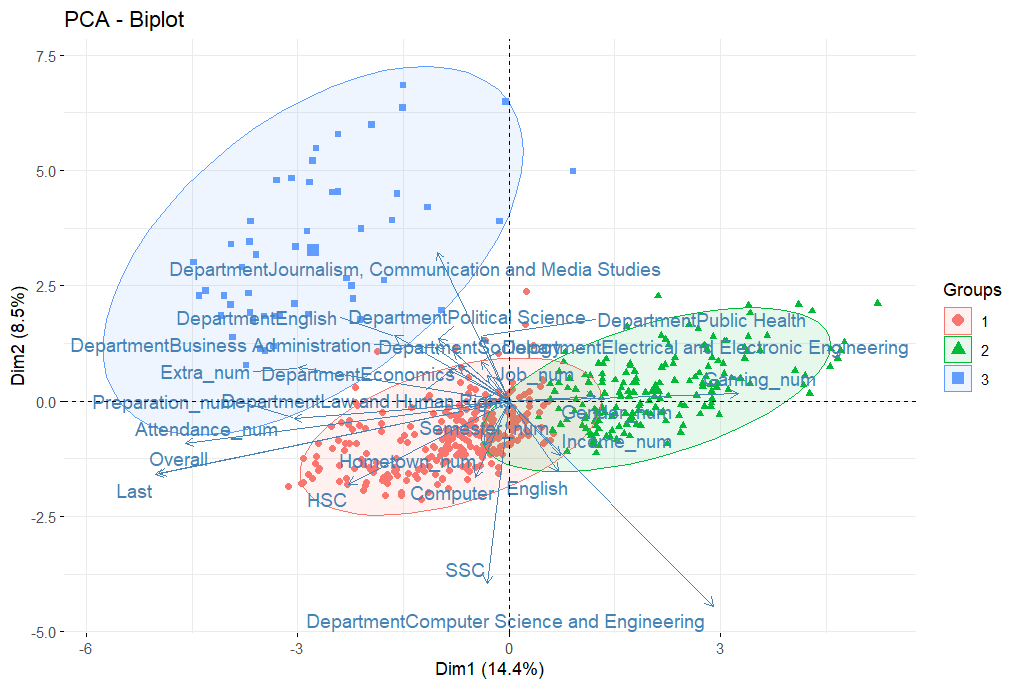
\includegraphics[width=0.8\textwidth]{figures/biplotcluttered.png}
    \caption{Contoh biplot dengan terlalu banyak fitur sehingga tampak berantakan}\label{fig:biplotcluttered}
\end{figure}

\begin{figure}[!htpb]
    \centering
    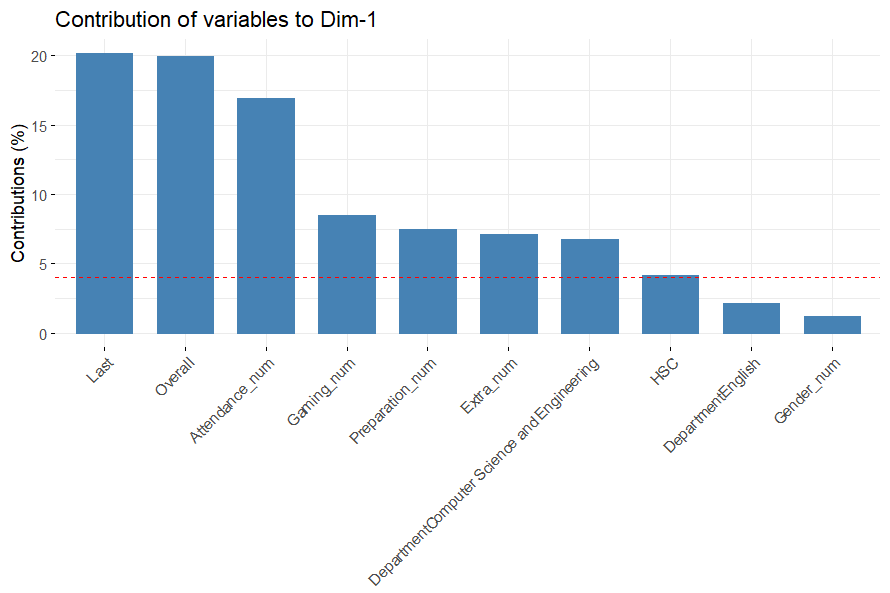
\includegraphics[width=0.8\textwidth]{figures/Dim1.png}
    \caption{Visualisasi kontribusi tiap fitur terhadap pembentukan cluster}
    \label{fig:cluster-contribution1}
\end{figure}

\begin{figure}[!htpb]
    \centering
    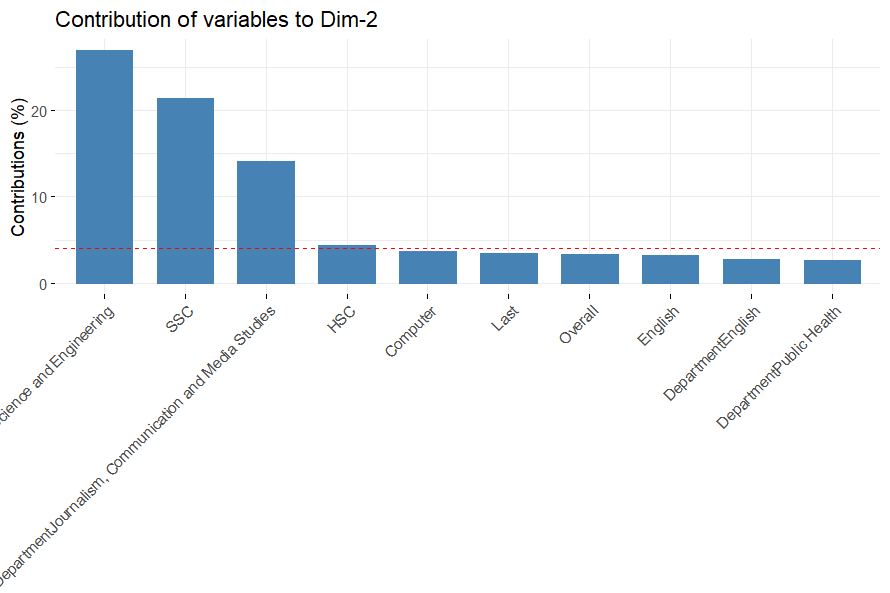
\includegraphics[width=0.8\textwidth]{figures/Dim2.png}
    \caption{Visualisasi kontribusi tiap fitur terhadap pembentukan cluster}
    \label{fig:cluster-contribution2}
\end{figure}

\begin{figure}[!htpb]
    \centering
    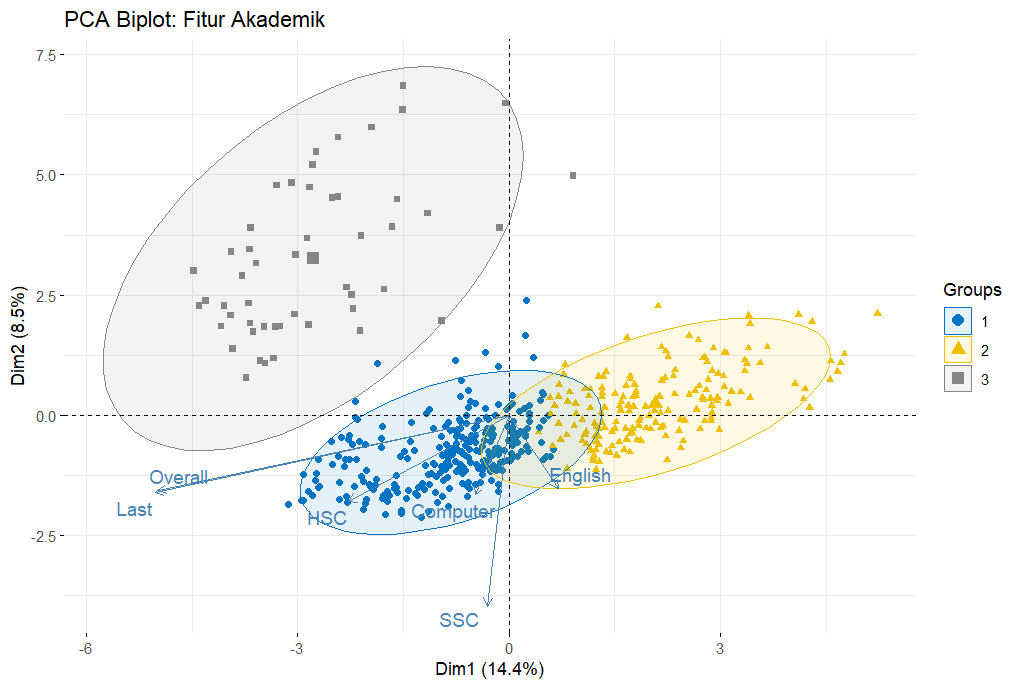
\includegraphics[width=0.8\textwidth]{figures/academicplot.png}
    \caption{Biplot fitur akademik}
    \label{fig:biplot-academic}
\end{figure}

\begin{figure}[!htpb]
    \centering
    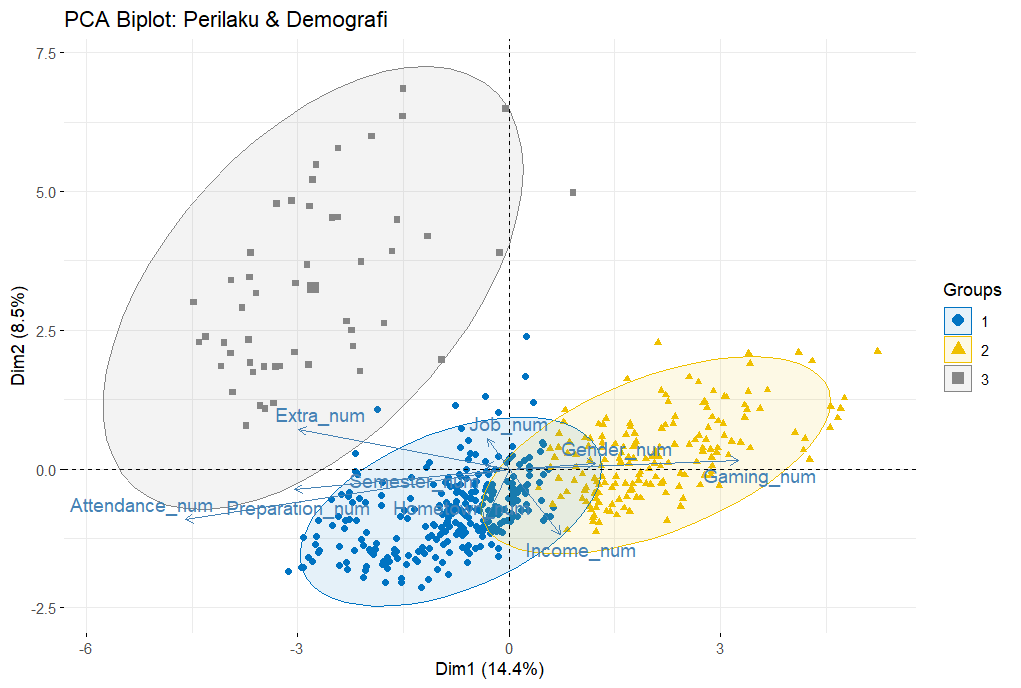
\includegraphics[width=0.8\textwidth]{figures/habitsplot.png}
    \caption{Biplot fitur perilaku dan demografi}
    \label{fig:biplot-habits}
\end{figure}

\begin{figure}[!htpb]
    \centering
    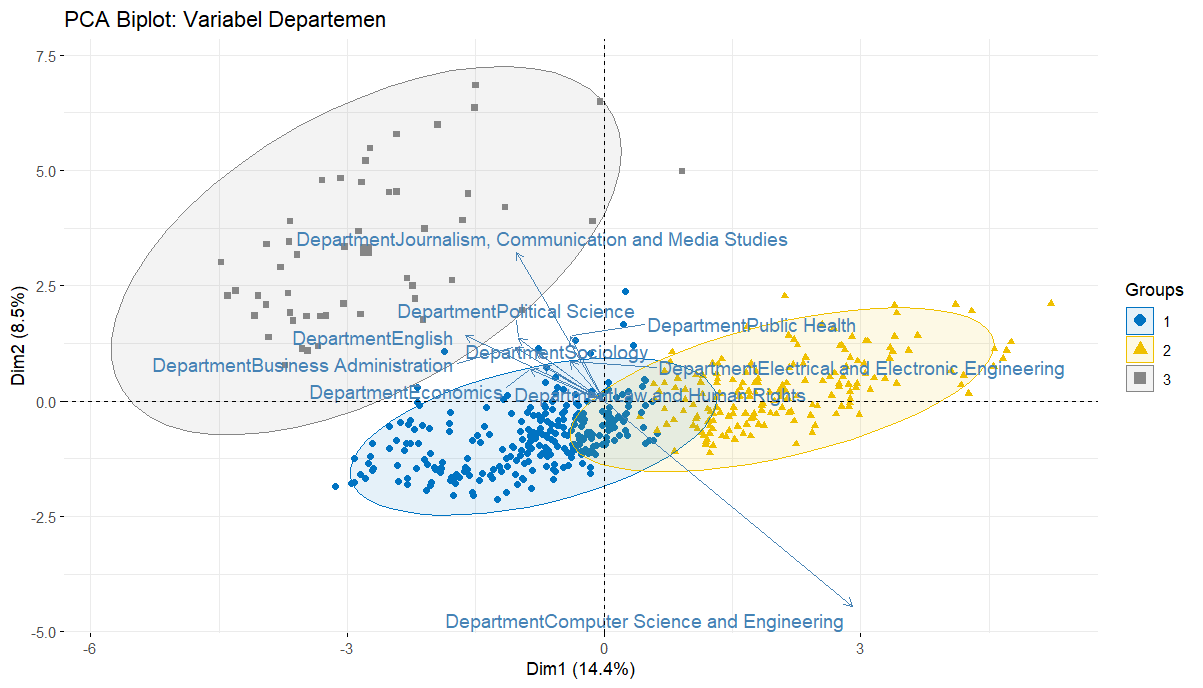
\includegraphics[width=0.8\textwidth]{figures/departmentplot.png}
    \caption{Biplot variabel departemen}
    \label{fig:biplot-department}
\end{figure}

\pagebreak
\subsection{Evaluasi Clustering}
\begin{figure}[!htpb]
    \centering
    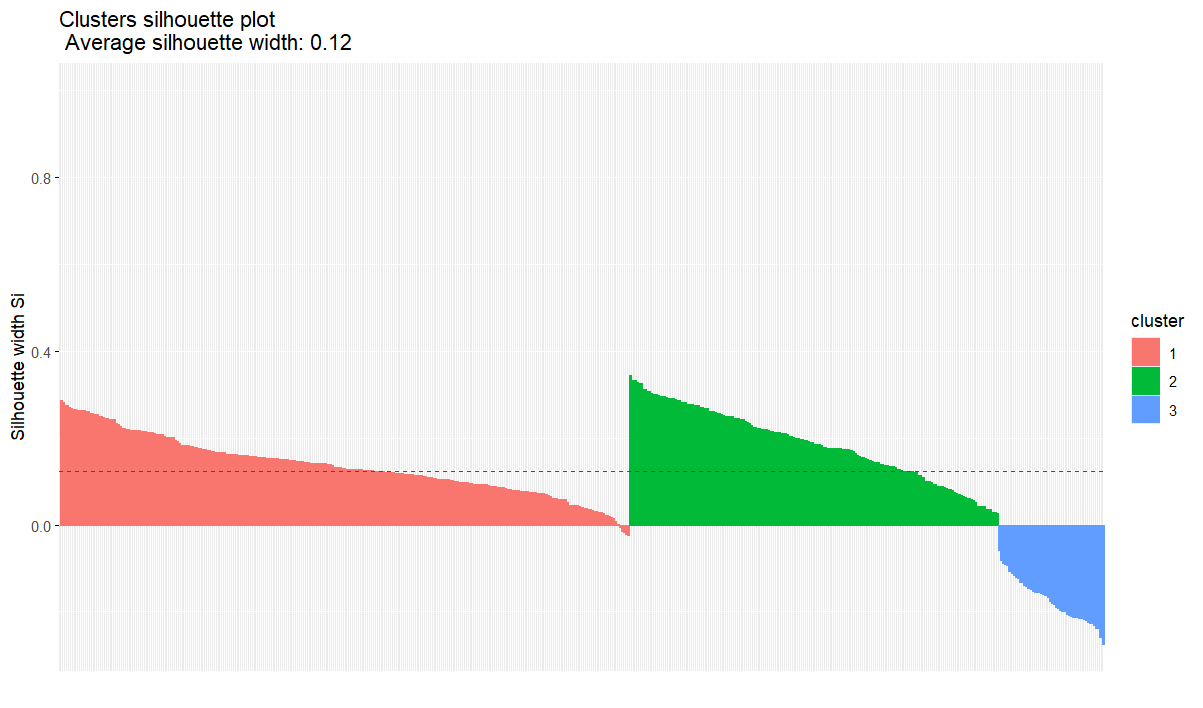
\includegraphics[width=0.8\textwidth]{figures/silhouetteplot.png}
    \caption{Silohutte plot}
    \label{fig:silhouetteplot}
\end{figure}
Evaluasi hasil clustering dilakukan menggunakan metode Silhouette Analysis. Rata-rata nilai silhouette width yang diperoleh sebesar 0.12, menandakan pemisahan antar klaster masih kurang kuat dan terdapat potensi tumpang tindih antar anggota klaster. Hal ini mengindikasikan bahwa hasil klasterisasi K-Means belum sepenuhnya mencerminkan struktur alami data.

Meskipun demikian, berdasarkan Elbow Method dan Gap Statistic (Grafik~\ref{fig:elbowmethod} dan Grafik~\ref{fig:gapstat}), jumlah klaster optimal tetap berada pada angka 3, sehingga K-Means masih dapat digunakan sebagai dasar segmentasi awal. Validasi tambahan melalui visualisasi PCA biplot juga memperlihatkan adanya pemisahan klaster, meskipun tidak terlalu tegas. Untuk memperoleh hasil yang lebih baik, metode clustering lain seperti Hierarchical Clustering atau DBSCAN dapat dipertimbangkan sebagai alternatif perbandingan.
\subsection{Evaluasi PCA}
\begin{figure}[!htpb]
    \centering
    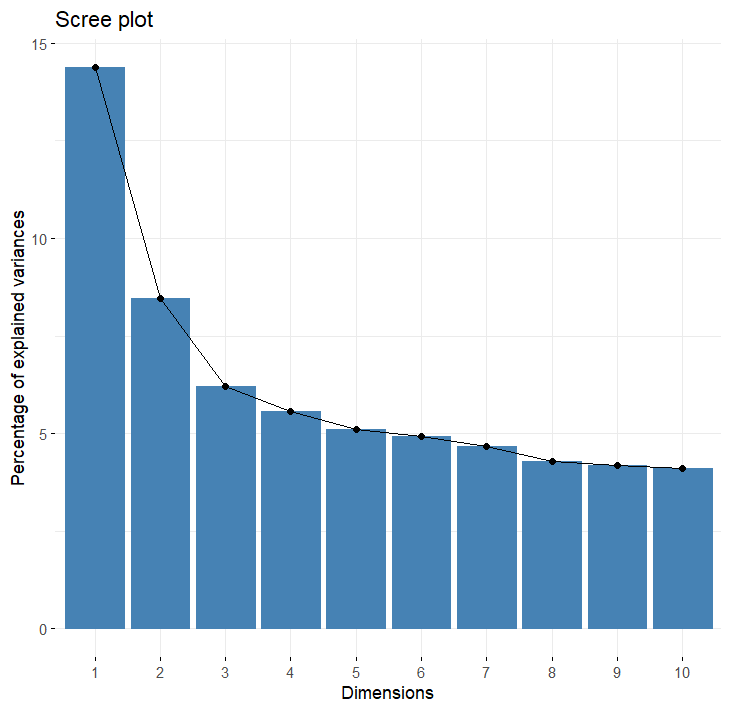
\includegraphics[width=0.8\textwidth]{figures/screeplot.png}
    \caption{Scree plot}
    \label{fig:screeplot}
\end{figure}
\begin{table}[!htpb]
    \centering
    \caption{Hasil PCA: Proporsi Variansi pada Komponen Utama}
    \label{tab:pca-variance}
    \begin{tabular}{lcccc}
        \hline
        \textbf{Komponen Utama} & \textbf{Simpangan Baku} & \textbf{Proporsi Variansi} & \textbf{Akumulasi Variansi} \\
        \hline
        PC1 & 1.8960 & 14.38\% & 14.38\% \\
        PC2 & 1.4549 & 8.47\% & 22.85\% \\
        PC3 & 1.2471 & 6.22\% & 29.07\% \\
        PC4 & 1.1790 & 5.56\% & 34.63\% \\
        PC5 & 1.1291 & 5.10\% & 39.73\% \\
        PC6 & 1.1098 & 4.93\% & 44.65\% \\
        PC7 & 1.0806 & 4.67\% & 49.33\% \\
        PC8 & 1.0358 & 4.29\% & 53.62\% \\
        \hline
    \end{tabular}
\end{table}

Berdasarkan Grafik~\ref{fig:screeplot}, terlihat adanya elbow pada dimensi ke-3. Namun, Tabel~\ref{tab:pca-variance} menunjukkan bahwa diperlukan delapan komponen utama (PC1–PC8) untuk menjelaskan lebih dari 50\% total variansi. Hal ini mengindikasikan bahwa tidak terdapat satu atau dua komponen yang secara dominan merepresentasikan data, sehingga variansi tersebar pada banyak dimensi. Dengan demikian, visualisasi PCA dua dimensi (PC1 vs PC2) memang kurang mampu menangkap keseluruhan struktur data, namun tetap bermanfaat untuk eksplorasi awal pola klaster dan arah kontribusi variabel.
\pagebreak
\subsection{Pembahasan}
Hasil analisis menunjukkan bahwa mahasiswa dalam dataset dapat dikelompokkan ke dalam tiga klaster utama, meskipun pemisahan antar klaster masih kurang tegas sebagaimana tercermin dari nilai silhouette yang rendah (0.12). Hal ini mengindikasikan adanya kompleksitas struktur data yang belum sepenuhnya terakomodasi oleh metode K-Means, kemungkinan akibat adanya tumpang tindih antar variabel atau hubungan non-linier antar fitur.

Meskipun demikian, hasil clustering yang dihasilkan model (lihat Grafik~\ref{fig:cluster-visualization-png}) tetap dapat diinterpretasikan sebagai berikut:
\begin{itemize}
    \item Klaster biru didominasi oleh mahasiswa dari "Department Computer Science and Engineering" dengan performa akademik tinggi. Berdasarkan Tabel~\ref{tab:cluster-distribusi}, klaster 1 berisi mahasiswa dengan GPA $\geq$ 3{,}5, tingkat kehadiran baik, frekuensi bermain game rendah, persiapan belajar optimal, serta kemampuan komputer yang baik.
    \item Klaster kuning juga didominasi oleh mahasiswa dari "Department Computer Science and Engineering", namun dengan performa akademik lebih rendah. Klaster ini mencakup mahasiswa dengan GPA sekitar 2, tingkat kehadiran rendah, frekuensi bermain game lebih tinggi, persiapan belajar kurang, serta kemampuan komputer yang sedang.
    \item Klaster merah terdiri dari mahasiswa dengan performa akademik tinggi, tingkat kehadiran dan persiapan belajar yang baik, namun kemampuan komputer relatif lebih rendah dibandingkan kedua klaster lainnya. Klaster ini umumnya berasal dari departemen non-STEM.
    \end{itemize}

Perlu dicatat bahwa GPA yang diamati merupakan indikator performa akademik yang dapat mengandung bias sistematis, sehingga kurang tepat jika dijadikan satu-satunya dasar untuk menilai ketimpangan penilaian. Analisis menggunakan model logistik terhadap GPA memberikan gambaran yang lebih komprehensif mengenai performa akademik. Ketika membandingkan mahasiswa dengan kemampuan akademik yang setara, ditemukan bahwa mahasiswa STEM cenderung memperoleh nilai dan GPA yang lebih rendah. Hal ini terutama disebabkan oleh standar penilaian yang lebih ketat pada mata kuliah STEM. Temuan ini sejalan dengan penelitian oleh \cite{Tomkin2022}, yang menunjukkan bahwa GPA mahasiswa non-STEM cenderung lebih tinggi dibandingkan mahasiswa STEM karena mata kuliah di bidang STEM umumnya memiliki tingkat kesulitan yang lebih tinggi.

Dari visualisasi PCA dan kontribusi fitur terhadap dimensi utama, didapati bahwa variabel "Gaming\_num" dan "Preparation\_num" memiliki hubungan yang signifikan terhadap nilai GPA "Overall". Mahasiswa dengan waktu bermain game yang tinggi cenderung memiliki nilai GPA yang lebih rendah, sedangkan mereka yang meluangkan waktu lebih banyak untuk persiapan belajar cenderung memiliki GPA yang lebih tinggi. Pola ini terlihat konsisten pada arah panah dalam biplot, di mana "Gaming\_num" berlawanan arah dengan "Overall" dan "Last", menunjukkan korelasi negatif. Sebaliknya, "Preparation\_num" cenderung searah dengan variabel akademik, mengindikasikan pengaruh positif terhadap performa.

Temuan ini juga sejalan dengan hasil penelitian eksperimental oleh \cite{Weis2010}, yang menunjukkan bahwa anak laki-laki yang diberikan akses ke video game cenderung menghabiskan lebih banyak waktu untuk bermain dan lebih sedikit waktu untuk aktivitas akademik setelah sekolah. Studi tersebut menemukan bahwa kelompok yang langsung menerima konsol video game memiliki skor membaca dan menulis yang lebih rendah serta lebih banyak masalah akademik menurut laporan guru dibandingkan kelompok kontrol. Selain itu, durasi bermain video game terbukti menjadi mediator antara kepemilikan video game dan penurunan hasil akademik. Hasil ini memberikan bukti bahwa video game dapat menggantikan waktu untuk aktivitas edukatif dan berpotensi menghambat perkembangan keterampilan membaca dan menulis pada anak-anak.

Temuan ini semakin menegaskan bahwa perilaku belajar dan pengelolaan waktu, khususnya terkait kebiasaan bermain game dan persiapan belajar, berperan penting dalam pencapaian akademik mahasiswa. Selain faktor akademik, variabel seperti departemen dan latar belakang demografis juga berkontribusi terhadap pembentukan klaster, meskipun pengaruhnya tidak sebesar faktor perilaku.

Walaupun hasil clustering belum sepenuhnya optimal, pendekatan ini tetap memberikan gambaran awal yang bermanfaat untuk segmentasi mahasiswa. Informasi ini dapat dimanfaatkan institusi pendidikan untuk merancang intervensi yang lebih terarah, misalnya dengan memberikan dukungan tambahan kepada kelompok mahasiswa yang berada pada klaster dengan skor akademik rendah dan intensitas bermain game yang tinggi.

Ke depannya, penerapan metode klasterisasi alternatif seperti Hierarchical Clustering atau DBSCAN, serta penggunaan teknik reduksi dimensi non-linier seperti t-SNE atau UMAP, dapat dipertimbangkan untuk memperoleh klaster yang lebih representatif dan mudah diinterpretasikan.
